\chapter{Технико-экономическое обоснование проекта}
\label{chap:economy}

В данной главе проведена оценка экономической эффективности разработки узла инерциальной навигационной системы на базе МЭМС-датчиков для путеизмерительной тележки ЗАО \enquote{ПИК Прогресс}. Замена прецизионного оптического гироскопа и механического акселерометра на микромеханические датчики позволила снизить себестоимость узла навигации с примерно $1{,}5$ млн~руб. до 40 тыс.~руб., что делает серийный выпуск тележки рентабельным.

% -----------------------------------------------------------------------------

\section{Анализ затрат, связанных с реализацией проекта}
\label{sec:economy_costs}

\subsection{Постоянные затраты}
\label{subsec:fixed_costs}

Фонд оплаты труда (ФОТ) на этапе разработки рассчитан исходя из 12-месячного срока проекта с учётом страховых взносов 30~\%. Состав группы разработчиков и распределение трудозатрат приведены в таблице~\ref{table:economy_payroll}.

\begin{table}[ht]
	\centering
	\small
	\begin{tabular}{|l|r|r|r|r|}
		\hline
		Специалист 					& \makecell{Оклад,\\ тыс.~руб./мес.} & \makecell{Занятость,\\ \%} & \makecell{ФОТ,\\ тыс.~руб.} & \makecell{С взносами,\\ тыс.~руб.} \\
		\hline
		Конструктор 				& 100 & 50  & 600  & 780,00 \\
		Программист-электронщик 	& 45  & 100 & 540  & 702,00 \\
		Начальник отдела 			& 350 & 10  & 420  & 546,00 \\
		\hline
		\textbf{Итого} 				&     &     & \textbf{1\,560,00} & \textbf{2\,028,00} \\
		\hline
	\end{tabular}
	\caption{Фонд оплаты труда на этапе разработки проекта}
	\label{table:economy_payroll}
\end{table}

Накладные расходы приняты в размере 20~\% от ФОТ и составляют 405,60~тыс.~руб. Стоимость изготовления опытного образца рамы тележки оценена в 300,00~тыс.~руб.

Капитал, вложенный на этапе первоначальных инвестиций, определяется как сумма ФОТ с учётом страховых взносов, накладных расходов и стоимости опытного образца:

\begin{equation}
	IC = 2\,028{,}00 + 405{,}60 + 300{,}00 = 2\,733{,}60 \text{ тыс. руб.}
	\label{eq:economy_IC}
\end{equation}

\subsection{Переменные затраты}
\label{subsec:variable_costs}

Состав себестоимости комплектующих одной серийной тележки приведён в таблице~\ref{table:economy_unit_cost}.

\begin{table}[ht]
	\centering
	\small
	\begin{tabular*}{\textwidth}{@{\extracolsep{\fill}}|l|r|@{}}
		\hline
		Наименование 										& Стоимость, тыс.~руб. 	\\
		\hline
		Конструкционная рама 								& 100 					\\
		Блок МЭМС и МК (разрабатываемый узел) 				& 40 					\\
		Блок датчиков пройденного пути 						& 10 					\\
		Блок датчиков ширины колеи 							& 10 					\\
		Бортовой компьютер 									& 50 					\\
		Аккумуляторная батарея 								& 10 					\\
		\hline
		\textbf{Итого} 										& \textbf{220} 			\\
		\hline
	\end{tabular*}
	\caption{Себестоимость комплектующих одной путеизмерительной тележки}
	\label{table:economy_unit_cost}
\end{table}

% -----------------------------------------------------------------------------

\section{Расчёт финансовых показателей}
\label{sec:economy_financial}

Параметры проекта приняты следующие: цена продажи одной тележки --- 3\,000~тыс.~руб., себестоимость комплектующих --- 220~тыс.~руб., плановая производственная мощность --- 10 шт./год, график освоения мощности --- 30/60/100~\% (3, 6 и 10 шт. по годам соответственно). Постоянные операционные затраты на этапе серийного производства (ФОТ сопровождения, принятый равным 20~\% от исходного, плюс накладные расходы) составляют 486,72~тыс.~руб./год.

\subsection{Доход}
\label{subsec:revenue}

Выручка формируется за счёт продаж путеизмерительных тележек нового поколения, серийный выпуск которых стал возможным благодаря удешевлению узла навигации. Расчёт выручки по годам приведён в таблице~\ref{table:economy_revenue}.

\begin{table}[ht]
	\centering
	\small
	\begin{tabular*}{\textwidth}{@{\extracolsep{\fill}}|c|r|r|r|@{}}
		\hline
		Год 	& Количество, шт. 	& Цена, тыс.~руб. 	& Выручка, тыс.~руб. 	\\
		\hline
		1 		& 3 				& 3\,000 			& 9\,000 				\\
		2 		& 6 				& 3\,000 			& 18\,000 				\\
		3 		& 10 				& 3\,000 			& 30\,000 				\\
		\hline
	\end{tabular*}
	\caption{Выручка от продаж путеизмерительных тележек по годам}
	\label{table:economy_revenue}
\end{table}

\subsection{Экономия}
\label{subsec:savings}

Экономия на комплектующих за счёт замены оптического гироскопа и механического акселерометра на МЭМС-датчики составляет $1\,500 - 40 = 1\,460$~тыс.~руб. на одну тележку. Совокупная экономия по годам приведена в таблице~\ref{table:economy_savings}.

\begin{table}[ht]
	\centering
	\small
	\begin{tabular*}{\textwidth}{@{\extracolsep{\fill}}|c|r|r|r|@{}}
		\hline
		Год 	& Количество, шт. 	& Экономия на единицу, тыс.~руб. 	& Экономия за год, тыс.~руб. 	\\
		\hline
		1 		& 3 				& 1\,460 							& 4\,380 						\\
		2 		& 6 				& 1\,460 							& 8\,760 						\\
		3 		& 10 				& 1\,460 							& 14\,600 						\\
		\hline
	\end{tabular*}
	\caption{Экономия на комплектующих за счёт применения МЭМС-датчиков}
	\label{table:economy_savings}
\end{table}

% -----------------------------------------------------------------------------

\section{Оценка эффективности предлагаемых мероприятий}
\label{sec:economy_efficiency}

\subsection{Ставка дисконтирования}
\label{subsec:discount_rate}

Ставка дисконтирования выбрана по методике Я.~Хонко для категории <<инвестиции для получения дохода (новые проекты на стабильном рынке)>> и принята равной $i = 20~\%$.

Обоснование: проект относится к выводу нового продукта на действующий рынок путеизмерительной техники в Российской Федерации, где существуют устойчивые производители-аналоги (АО <<Фирма ТВЭМА>> и др.). Технологический риск проекта невысок, поскольку применяемые МЭМС-датчики серийно производятся и массово используются в смежных отраслях.

\subsection{Чистый денежный поток}
\label{subsec:cash_flow}

Ставка налога на прибыль организаций принята равной 25~\%. Расчёт денежных потоков по периодам приведён в таблице~\ref{table:economy_cash_flow}.

\begin{table}[H]
	\centering
	\small
	\begin{tabular*}{\textwidth}{@{\extracolsep{\fill}}|l|r|r|r|r|@{}}
		\hline
		Период, тыс.~руб. 										& Год 0 			& Год 1 			& Год 2 			& Год 3 			\\
		\hline
		\multicolumn{5}{|l|}{\textit{Приток}} 																									\\
		\hline
		Выручка от продаж 										& 0 				& 9\,000 			& 18\,000 			& 30\,000 			\\
		\hline
		\multicolumn{5}{|l|}{\textit{Отток}} 																									\\
		\hline
		Капитал первоначальных инвестиций 						& 2\,733,60 		& 0 				& 0 				& 0 				\\
		Переменные затраты 										& 0 				& 660 				& 1\,320 			& 2\,200 			\\
		Постоянные затраты 										& 0 				& 486,72 			& 486,72 			& 486,72 			\\
		Налог на прибыль (25~\%) 								& 0 				& 1\,963,32 		& 4\,048,32 		& 6\,828,32 		\\
		\hline
		\textbf{Чистый денежный поток} 							& \textbf{$-2\,733,60$} 	& \textbf{5\,889,96} 	& \textbf{12\,144,96} 	& \textbf{20\,484,96} 	\\
		\hline
		Коэффициент дисконтирования $1/(1+i)^k$ 				& 1,0000 			& 0,8333 			& 0,6944 			& 0,5787 			\\
		Дисконтированный денежный поток 						& $-2\,733,60$ 		& 4\,908,30 		& 8\,434,00 		& 11\,854,72 		\\
		\hline
		\textbf{Накопленный дисконтированный поток} 			& $-2\,733,60$ 		& 2\,174,70 		& 10\,608,70 		& \textbf{22\,463,42} 	\\
		\hline
	\end{tabular*}
	\caption{Денежные потоки проекта по периодам}
	\label{table:economy_cash_flow}
\end{table}

\subsection{Расчёт NPV}
\label{subsec:npv}

Чистая приведённая стоимость проекта рассчитывается по формуле:

\begin{equation}
	NPV = \sum_{k=1}^{n} \frac{P_k}{(1+i)^k} - IC,
	\label{eq:economy_npv}
\end{equation}

где $n = 3$ --- расчётный горизонт проекта, лет;
$P_k$ --- чистый денежный поток за $k$-й интервал времени;
$i = 0{,}20$ --- ставка дисконтирования;
$IC = 2\,733{,}60$~тыс.~руб. --- капитал, вложенный на этапе первоначальных инвестиций.

Подстановка значений в выражение~\eqref{eq:economy_npv} даёт:

\begin{equation}
	NPV = \frac{5\,889{,}96}{1{,}20} + \frac{12\,144{,}96}{1{,}44} + \frac{20\,484{,}96}{1{,}728} - 2\,733{,}60
	\label{eq:economy_npv_subst}
\end{equation}

\begin{equation}
	NPV = 4\,908{,}30 + 8\,434{,}00 + 11\,854{,}72 - 2\,733{,}60 \approx 22\,463 \text{ тыс. руб.} \text{ млн руб.}
	\label{eq:economy_npv_value}
\end{equation}

Поскольку $NPV > 0$, проект является прибыльным и приносит больше дохода, чем альтернативные вложения под выбранную ставку дисконтирования.

% -----------------------------------------------------------------------------

\section{Обоснование и поиск источников финансирования}
\label{sec:economy_funding}

\subsection{Информация о предприятии-заказчике}
\label{subsec:company_info}

Предприятием-заказчиком разработки выступает ЗАО <<ПИК Прогресс>>. Основные реквизиты компании приведены ниже:

\begin{table}[h!]
	\centering
	\begin{tabular}{>{\centering\arraybackslash}l l p{8cm}}
		Полное наименование 	& --- & ЗАКРЫТОЕ АКЦИОНЕРНОЕ ОБЩЕСТВО \enquote{ПИК ПРОГРЕСС}; \\
		Сокращённое наименование & --- & ЗАО \enquote{ПИК ПРОГРЕСС}; \\
		ОГРН 					& --- & 1027739713407; \\
		Дата регистрации 		& --- & 08.12.1994. \\
	\end{tabular}
\end{table}

\subsection{Анализ финансовых результатов компании}
\label{subsec:company_financial}

Финансовые показатели компании за 2022--2024~гг., полученные из электронного сервиса ФНС России <<Прозрачный бизнес>>, приведены в таблице~\ref{table:economy_company_financial}.

\begin{table}[ht]
	\centering
	\small
	\begin{tabular*}{\textwidth}{@{\extracolsep{\fill}}|l|r|r|r|r|r|r|r|@{}}
		\hline
		\multirow{2}{*}{\makecell[l]{Показатель,\\ тыс.~руб.}} 	& \multicolumn{3}{c|}{Значение} 	& \multicolumn{2}{c|}{Абс. откл.} 	& \multicolumn{2}{c|}{Отн. откл., \%} 	\\
		\cline{2-8}
		& 2022 				& 2023 				& 2024 				& 23/22 			& 24/23 			& 23/22 			& 24/23 			\\
		\hline
		Выручка 								& 263\,174 			& 536\,389 			& 323\,070 			& $+273\,215$ 		& $-213\,319$ 		& $+103{,}8$ 		& $-39{,}8$ 		\\
		\hline
		\makecell[l]{Себестоимость\\ продаж} 	& 238\,126 			& 435\,242 			& 270\,153 			& $+197\,116$ 		& $-165\,089$ 		& $+82{,}8$ 		& $-37{,}9$ 		\\
		\hline
		Прибыль 								& 25\,048 			& 101\,147 			& 52\,917 			& $+76\,099$ 		& $-48\,230$ 		& $+303{,}8$ 		& $-47{,}7$ 		\\
		\hline
	\end{tabular*}
	\caption{Финансовые результаты ЗАО \enquote{ПИК Прогресс} за 2022--2024~гг.}
	\label{table:economy_company_financial}
\end{table}

\begin{figure}[H]
	\centering
	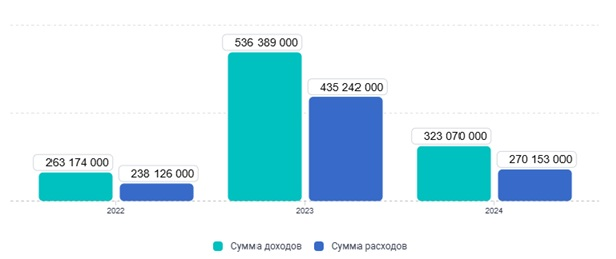
\includegraphics[width=0.8\textwidth]{images/Доходы ПИК Прогресс.jpg}
	\caption{Суммы доходов и расходов по данным бухгалтерской отчетности организации}
\end{figure}


Финансовые результаты компании свидетельствуют о стабильном функционировании предприятия на рынке с положительной прибылью на протяжении всех трёх анализируемых периодов.

\subsection{Источники финансирования проекта}
\label{subsec:funding_sources}

Объём капитала, вложенного на этапе первоначальных инвестиций (2,73 млн~руб.), составляет ${\approx}5{,}2~\%$ прибыли ЗАО \enquote{ПИК Прогресс} за 2024~год. Проект рекомендуется финансировать за счёт собственных средств предприятия: такой подход сохраняет финансовую независимость компании и исключает процентные платежи по заёмному капиталу.

% -----------------------------------------------------------------------------

\section*{Выводы по главе}
\addcontentsline{toc}{section}{Выводы по главе}

В рамках технико-экономического обоснования проекта получены следующие результаты:

\begin{enumerate}
	\item Капитал, вложенный на этапе первоначальных инвестиций, составил $IC = 2\,733{,}60$~тыс.~руб.
	
	\item Себестоимость комплектующих одной тележки --- 220~тыс.~руб., цена продажи --- 3\,000~тыс.~руб.
	
	\item Чистая приведённая стоимость проекта при ставке дисконтирования 20~\% и расчётном горизонте 3~года составила $NPV = 22{,}46$~млн~руб. (${>}0$), что свидетельствует о прибыльности проекта.
	
	\item Источником финансирования проекта приняты собственные средства ЗАО \enquote{ПИК Прогресс}.
\end{enumerate}

Разработанное решение на базе микромеханических датчиков является экономически целесообразным и обеспечивает положительную чистую приведённую стоимость проекта.

